\section{Fazit und Ausblick}

\subsection{Fazit}
Ziel dieser Arbeit war die Entwicklung eines automatisierbaren Montagekonzepts zum Montieren und Vorspannen von SLC-Linearführungen unter kontrollierten Kraft-, Positions- und Drehmomentbedingungen. Gleichzeitig sollte das System variantenfähig ausgelegt sein und eine Prozessüberwachung der wesentlichen Montageparameter ermöglichen. Dieses Ziel wurde im Rahmen der Arbeit vollständig erreicht.

Das entwickelte Montagesystem ermöglicht das reproduzierbare Vorspannen der Linearführungen sowie die kontrollierte Durchführung der relevanten Montageprozesse. Alle eingesetzten Aktoren und Sensoren funktionieren wie vorgesehen und konnten im Rahmen von Einzeltests erfolgreich in Betrieb genommen werden. Die durchgeführten Validierungstests zeigen, dass die Positioniergenauigkeit sowie die Wiederholbarkeit der Achssysteme innerhalb der geforderten Toleranzen liegen. Auch die Mess- und Überwachungseinrichtungen für Kraft, Position und Drehmoment arbeiten zuverlässig und liefern konsistente Ergebnisse.

Die Variantenfähigkeit des Systems wurde durch die modulare mechanische Auslegung sowie die Verwendung bestehender Werkstückträger sichergestellt. Dadurch können unterschiedliche Baugrößen der SLC-Positionierer ohne grundlegende Anpassungen am System montiert werden. Die Prozessüberwachung ist grundsätzlich realisiert, da alle relevanten Sensoren und Aktoren angebunden und auslesbar sind.

Einschränkend ist festzuhalten, dass der Betrieb des Systems aktuell ausschließlich manuell erfolgt. Ein vollautomatisierter Ablauf wurde im Rahmen dieser Arbeit nicht umgesetzt. Dies ist insbesondere auf die begrenzte verfügbare Bearbeitungszeit zurückzuführen. Dennoch bildet das entwickelte System eine funktionsfähige und validierte Grundlage für eine weiterführende Automatisierung.

\subsection{Ausblick}
Aufbauend auf den Ergebnissen dieser Arbeit ergeben sich mehrere sinnvolle Erweiterungen und Optimierungsmöglichkeiten, um das Montagesystem in Richtung eines industriell einsetzbaren Gesamtsystems weiterzuentwickeln.

Ein wesentlicher nächster Schritt ist die Ausarbeitung und Umsetzung eines vollständigen Sicherheitskonzepts. Die Sicherheit wurde im Rahmen dieser Arbeit bewusst nicht betrachtet. Für einen späteren produktiven Einsatz wären unter anderem ein Not-Aus-Konzept, eine mechanische Einhausung des Systems sowie die Berücksichtigung relevanter allgemeiner Sicherheitsnormen erforderlich.

Des Weiteren sollte die elektrische Integration der Komponenten in einem Schaltschrank erfolgen. Zwar sind alle Komponenten bereits vollständig verdrahtet und funktionsfähig, aktuell befinden sich diese jedoch noch auf dem Arbeitstisch. Ein Schaltschrank würde eine strukturierte, sichere und wartungsfreundliche Unterbringung der Steuerungs- und Leistungskomponenten ermöglichen. Dies ist aus sicherheitstechnischen Gründen erforderlich, insbesondere wenn der Aufbau den Experimentalstatus verlassen und in einen dauerhaften oder erweiterten Betrieb überführt werden soll. Ein entsprechender Schaltplan wurde bereits erstellt und kann hierfür als Grundlage dienen.

\begin{figure}[H]
    \centering
    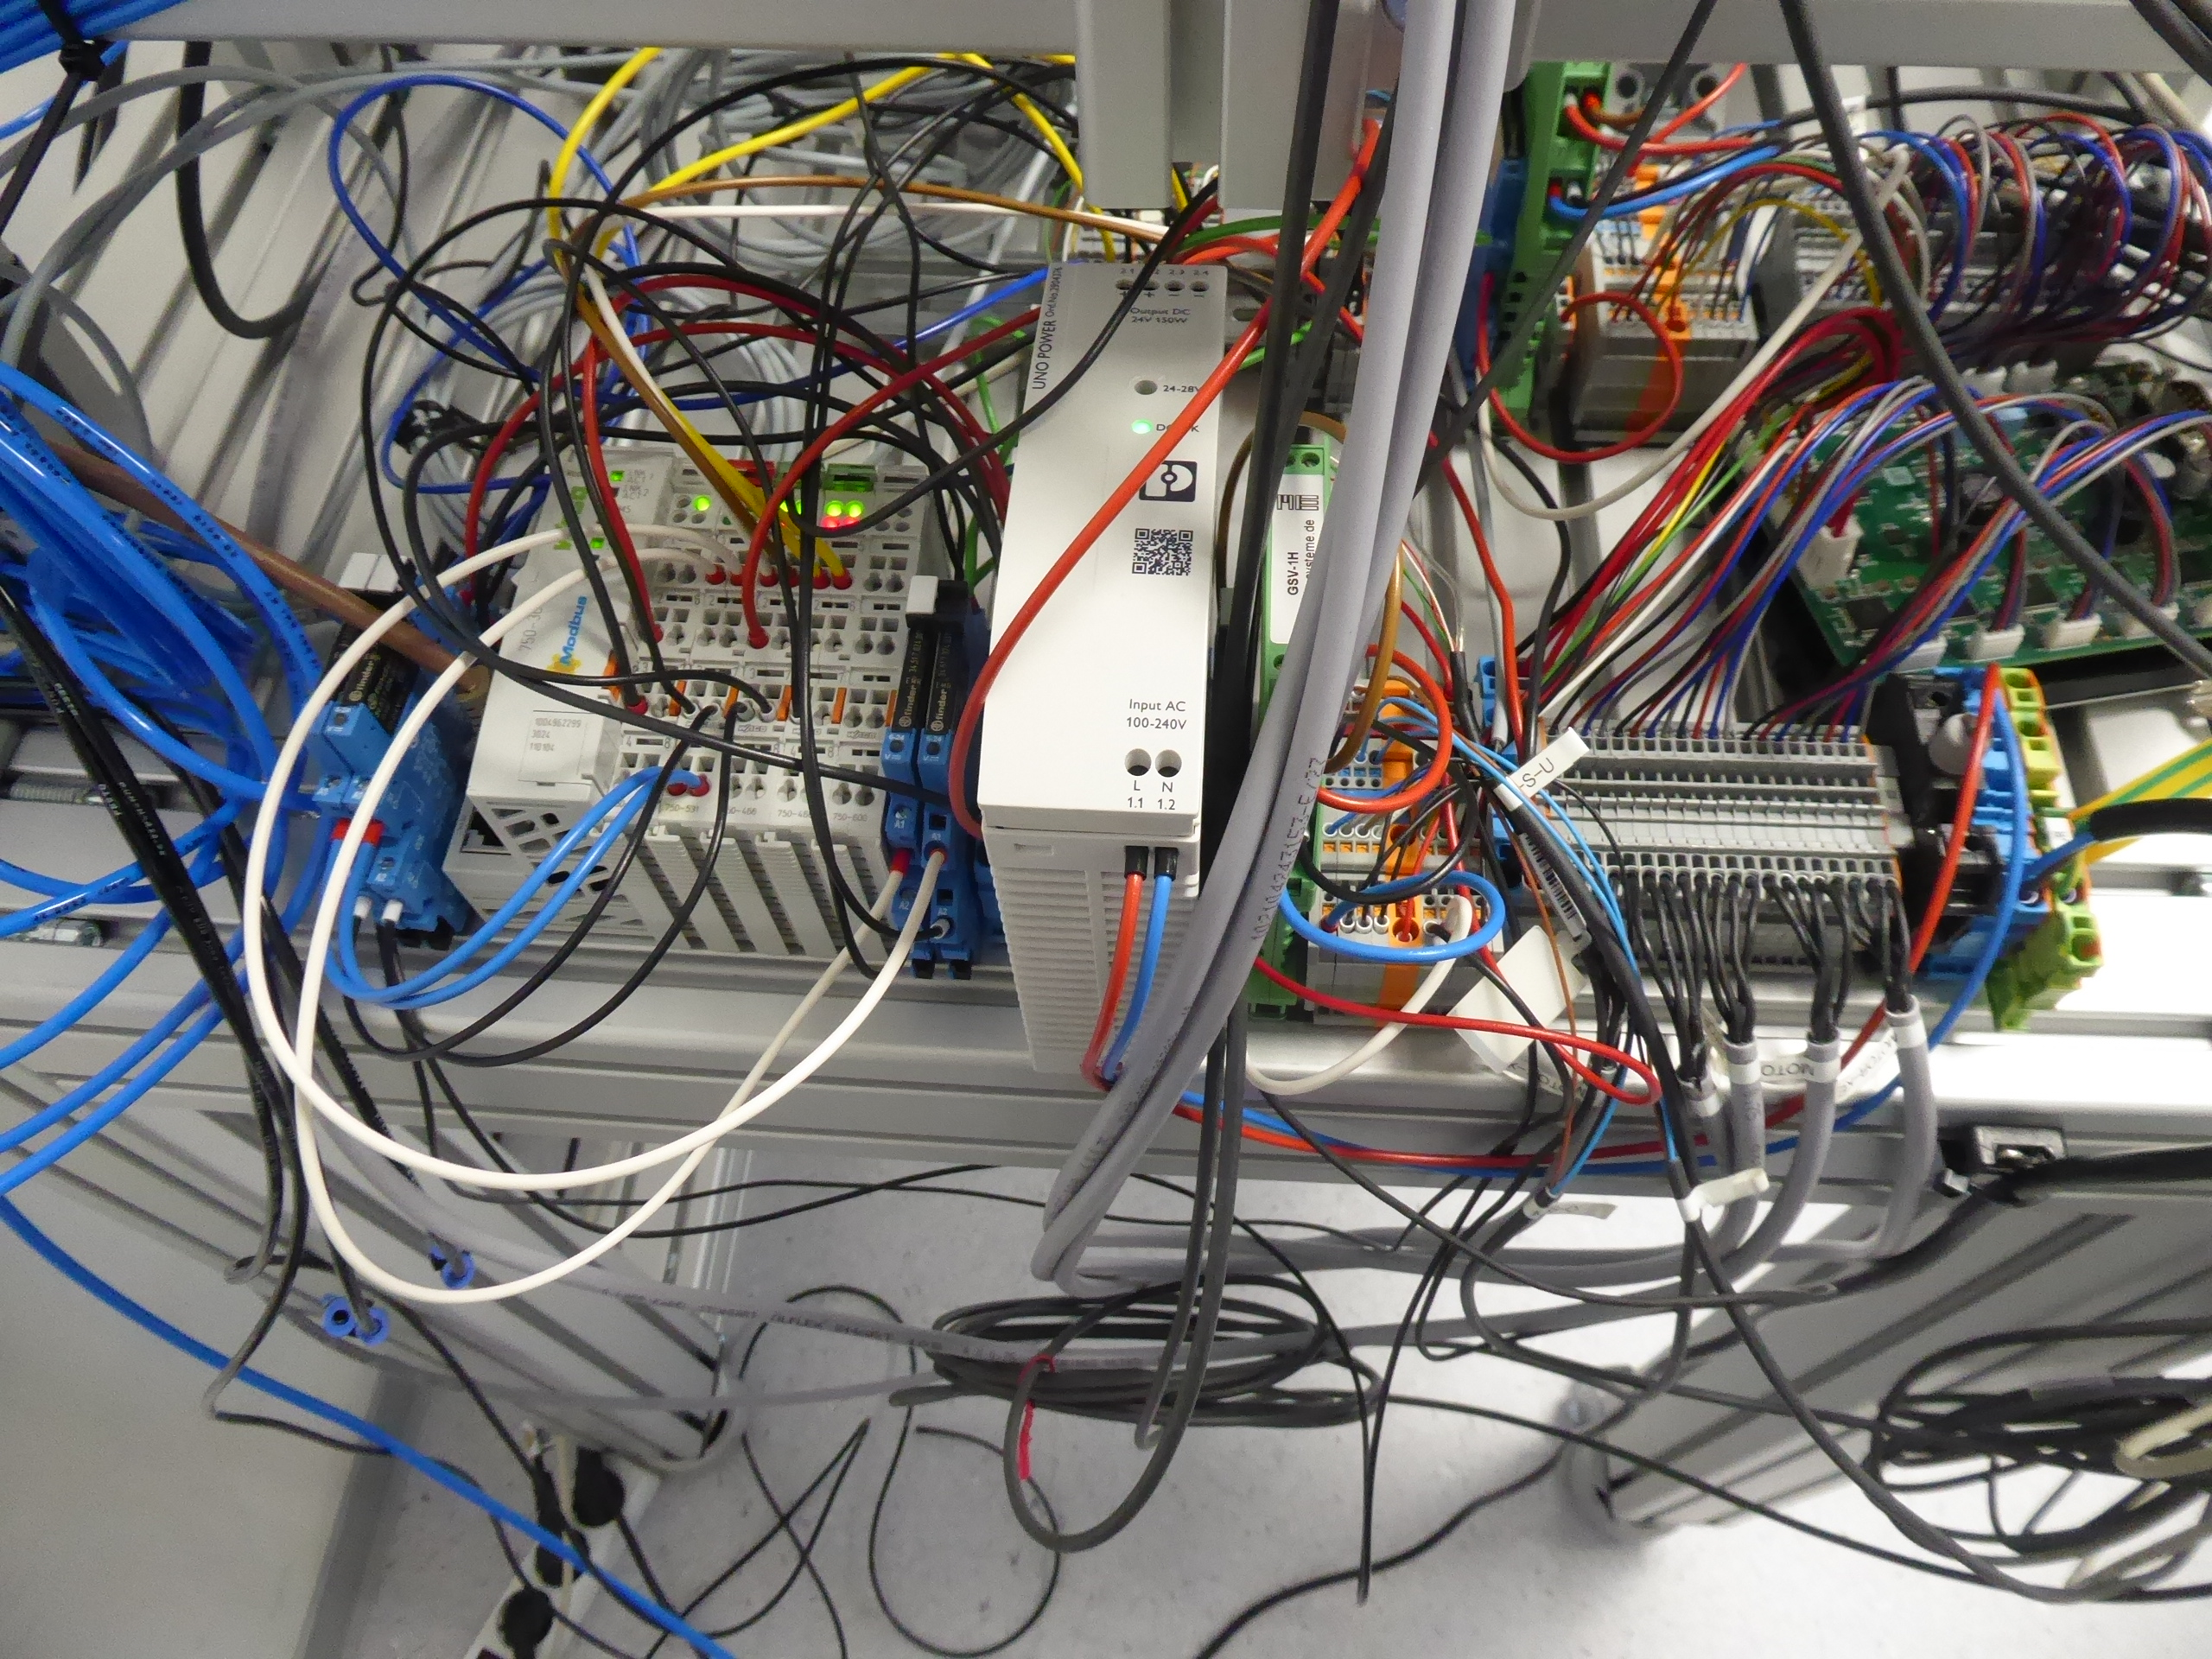
\includegraphics[width=0.5\textwidth]{Bilder/07_Fazit_und_Ausblick/Schaltschrank.JPG}
    \caption{Elektrische Komponenten außerhalb eines Schaltschranks}
\end{figure}

Ein weiterer zentraler Entwicklungsschritt betrifft die Software. Derzeit existieren lediglich Einzeltests ohne durchgängigen Automatisierungscode. Für den automatischen Betrieb wäre die Implementierung eines vollständigen Positionier- und Ablaufprogramms erforderlich. Dieses könnte beispielsweise auf einem PC-basierten System umgesetzt und über Python realisiert werden. Dabei müssten unter anderem Referenzfahrten, Bewegungsprofile, Zustandslogik sowie eine einfache Fehlerbehandlung implementiert werden.

Zusätzlich sollte die Kabelführung des Systems überarbeitet werden. Aktuell ist diese nur provisorisch ausgeführt. Für einen zuverlässigen Dauerbetrieb wären strukturierte Kabelführungen, beispielsweise in Form von Energieketten, sowie geeignete Zugentlastungen notwendig.

\begin{figure}[H]
    \centering
    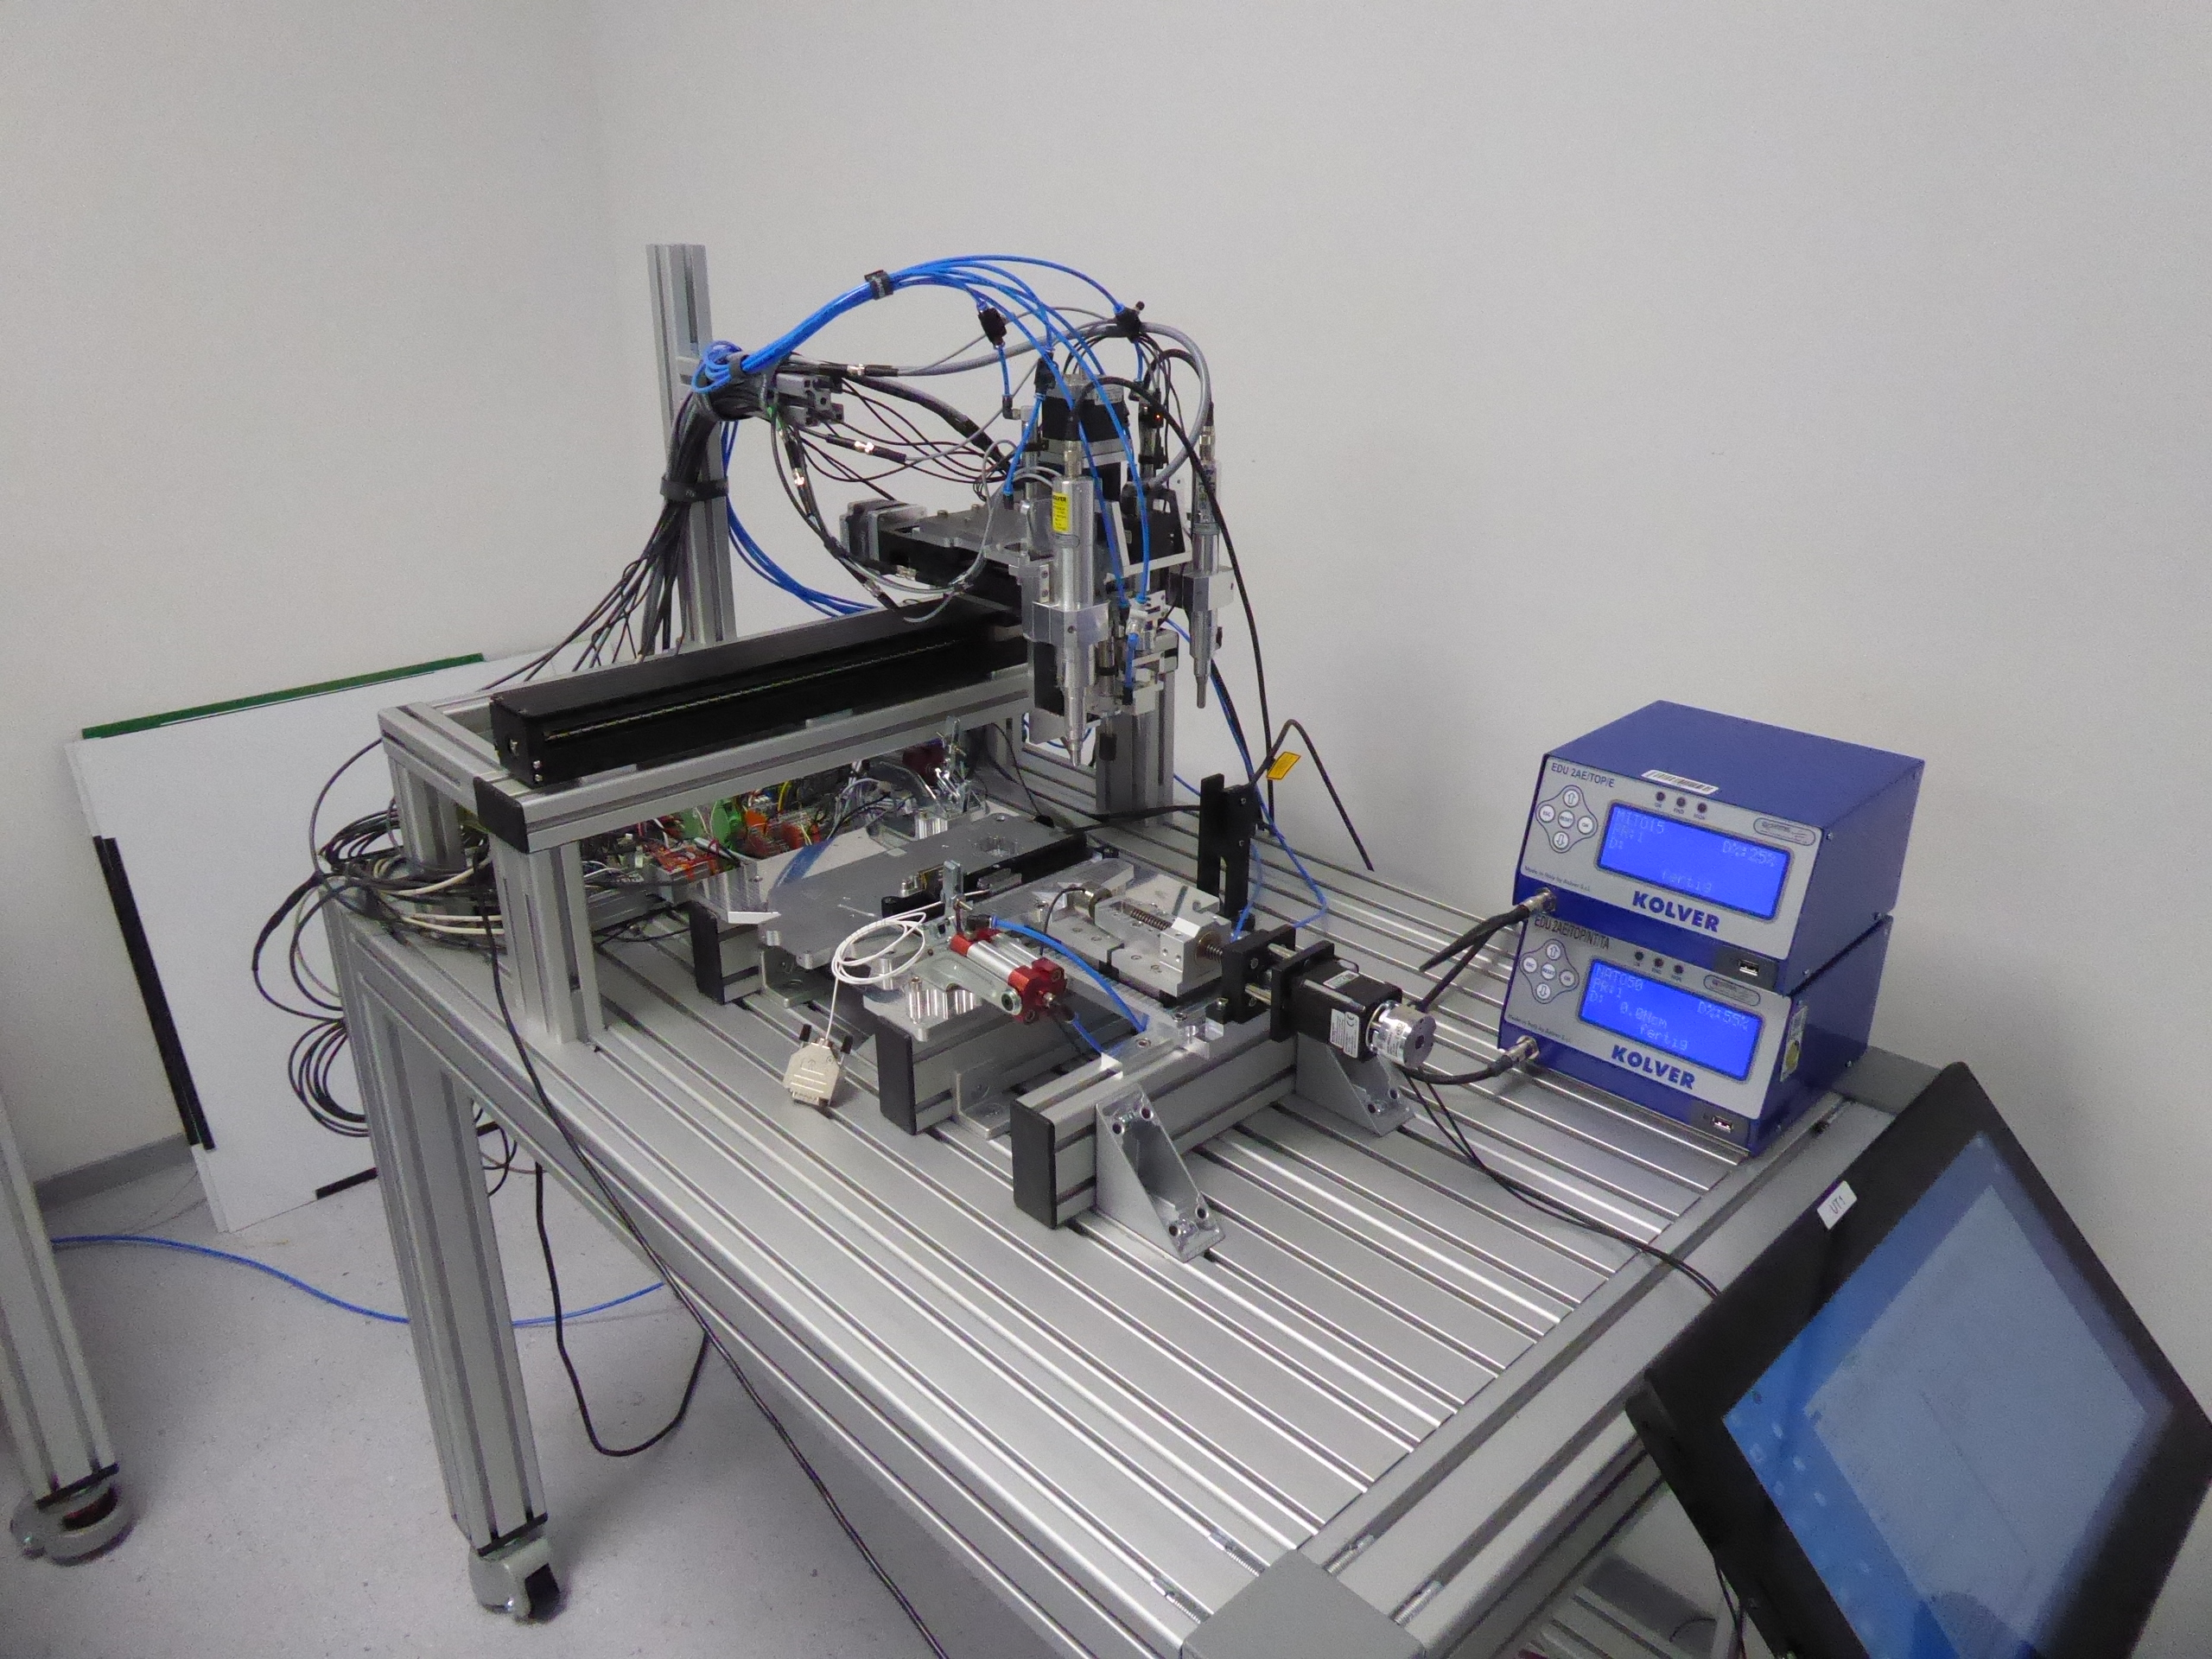
\includegraphics[width=0.5\textwidth]{Bilder/07_Fazit_und_Ausblick/kabelführung.JPG}
    \caption{Provisorische Kabelführung des Versuchsaufbaus}
\end{figure}

Insgesamt stellt das im Rahmen dieser Arbeit entwickelte Montagesystem eine stabile und funktionale Basis dar, auf der zukünftige Erweiterungen in Richtung Automatisierung, Sicherheit und Serienreife systematisch aufbauen können.